\documentclass{article}
\usepackage[T1]{fontenc}
\usepackage{lmodern}
\usepackage{graphicx}
\usepackage{amsmath,amssymb}
\usepackage[a4paper,margin=2cm]{geometry}
\usepackage[absolute,overlay]{textpos}
\setlength{\TPHorizModule}{1mm}
\setlength{\TPVertModule}{1mm}
\usepackage[indonesian]{babel}
\usepackage{hyperref}
\setlength{\emergencystretch}{2em}
% unit: Halaman 47

\begin{document}

% === Halaman 47 (llm) ===

\vspace{172.26mm}

Misalkan $\underline{\text{semua}}$ bit LSB pada citra $grayscale$ dibalikkan\\Dari semula 0 menjadi 1; dari semula 1 menjadi 0
\vspace{20mm}
\begin{center}
Sebelum \hspace{5cm} Sesudah
\end{center}
\begin{center}
\textcolor{red}{Adakah terlihat perbedaaanya?}
\end{center}

% deskripsi: Perbandingan dua citra grayscale sebuah gedung sebelum dan sesudah manipulasi bit LSB (Least Significant Bit), di mana citra kiri berlabel 'Sebelum' dan citra kanan berlabel 'Sesudah'.
% bbox normalisasi: [0.1500, 0.2300, 0.8500, 0.8100]
\begin{textblock*}{147.00mm}(31.50mm,68.31mm)
\noindent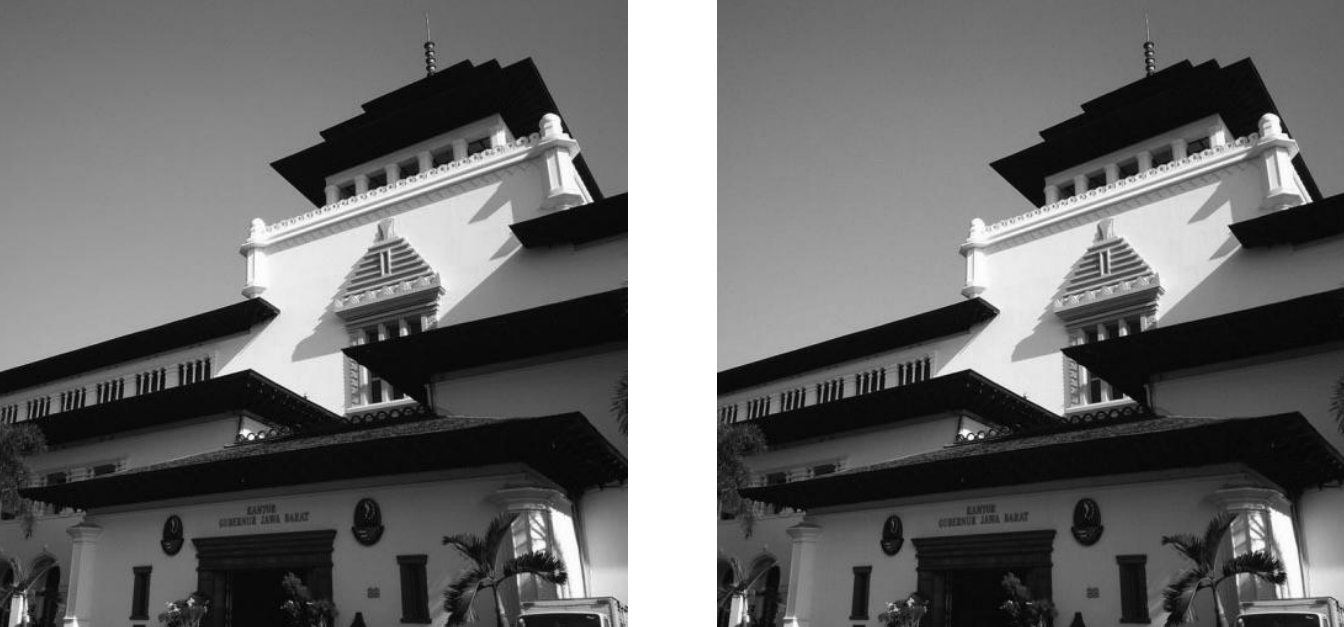
\includegraphics[width=147.00mm,height=172.26mm]{../../images/llm/page_047_img_01.png}%
\end{textblock*}

\end{document}
